\chapter{RDFRules Reference Implementation\label{rdfrules}}

\cite{Zeman2020} also presents an open-source implementation of the improved AMIE+ algorithm and some of the proposed supporting techniques\footnote{Unlike the reference implementation of the AMIE+ authors that focuses solely on the modelling phase.} as a single framework under the name RDFRules. The source code of the framework is available at \href{https://github.com/propi/rdfrules}{https://github.com/propi/rdfrules}. It can act as an equivalent to the modern algoritmic frameworks for mining association rules from tabular data, such as \textit{arules} R package or Spark MLlib that enable to deal with the whole mining process with just one tool.

\section{Interfaces}

The core of the framework is written in Scala. Beside the Scala API\footnote{\href{https://github.com/propi/rdfrules/tree/master/core}{https://github.com/propi/rdfrules/tree/master/core}}, the framework also provides a Java API\footnote{\href{https://github.com/propi/rdfrules/tree/master/java}{https://github.com/propi/rdfrules/tree/master/java}} serving as the facade into the Scala core, though it is already\footnote{The current version of the framework as of writing this is \textit{1.5.0} published on November 28th 2020.} pronounced deprecated. Both APIs are published\footnote{\href{https://jitpack.io/\#propi/rdfrules}{https://jitpack.io/\#propi/rdfrules}} in the JitPack package repository, so they can be easily added to a Scala or Java project as a dependency. The framework also has a REST API wrapping the Scala core that can either be used as is and be accessed through an HTTP client or through a GUI via a web broswer.

\begin{figure}[h]
\centering
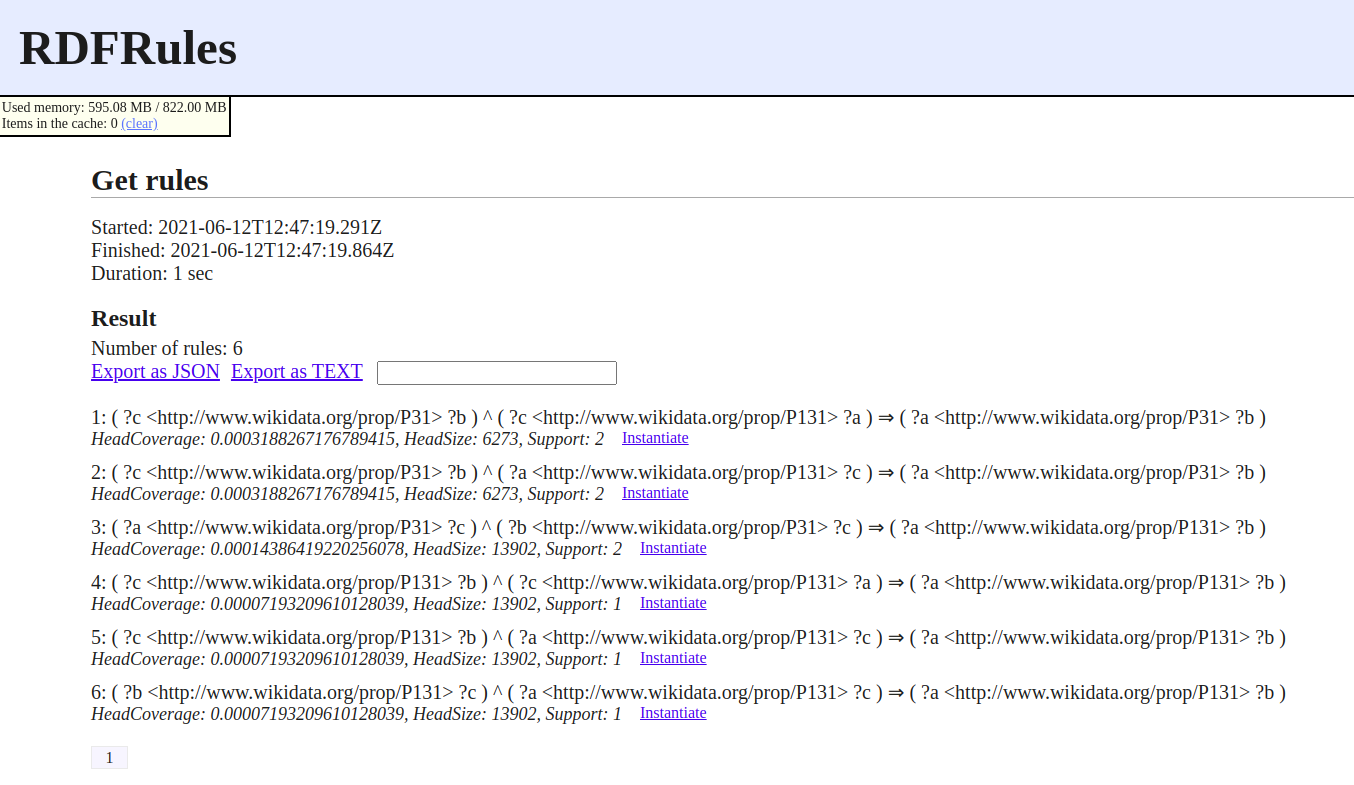
\includegraphics[width=0.8\textwidth]{img/gui-getrules.png}
\caption{RDFRules web browser interface}
\label{rdfrulesgui}
\end{figure}

\section{Data Structures}

The framework's core revolves around four main data structures: \textit{RDFGraph} and \textit{RDFDataset} corresponding to the input data, \textit{Index} wrapping the set of indices the input data is transformed into and \textit{RuleSet} containing rules generated by the algorithm. These structures are transformed into each other in the stated order during the mining process by applying various operations on them. Inspired by the Apache Spark RDD\footnote{\href{https://spark.apache.org/docs/latest/rdd-programming-guide.html\#resilient-distributed-datasets-rdds}{https://spark.apache.org/docs/latest/rdd-programming-guide.html\#resilient-distributed-datasets-rdds}} the operations are categorized into \textit{transformations} and \textit{actions}. All transformations are \textit{lazy} operations meaning they are not performed right after the API call but only when an action operation is called which is dependent on them.

Each transformation method called on an instance of the data structures returns either a modified version of the same instance or the instance transform into a further data structure but the instance which the method was called on does not change i.e. the objects of the framework are immutable and the whole workflow with the core API lies in chaining those methods. Multiple calls of an action operation with different input parameters would result in repetitive performance of the defined transformations so each data structure has a \textit{cache} method that enables preserving the result of the transformations in memory or on the disk so that they have to be performed only once.

\begin{figure}[h]
\centering
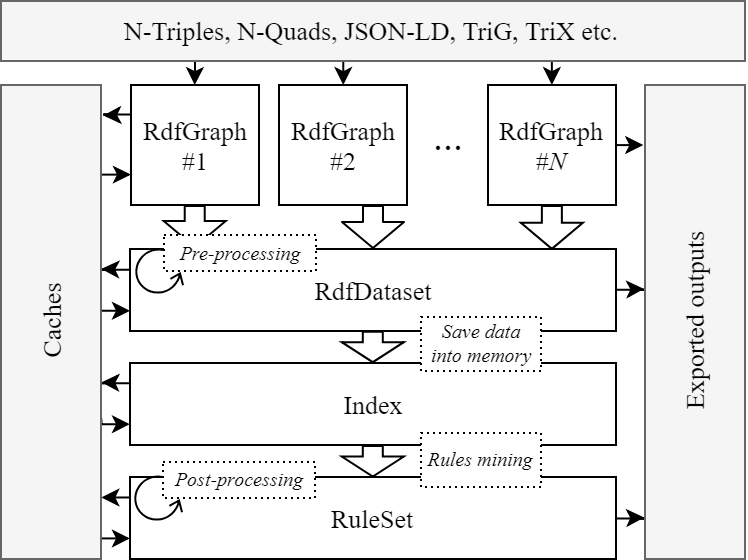
\includegraphics[width=0.6\textwidth]{img/rdfrules-abstractions.png}
\caption{Relations between the RDFRules data structures (Source: \cite{Zeman2018})}
\label{rdfrulesdatastructures}
\end{figure}

%\subsection{RDFGraph and RDFDataset}

An RDFGraph instance corresponds to a set of triples. It is created either from stream of triples or from a file containing a supported RDF serialization (N-Triples, N-Quads, JSON-LD, TriG, Turtle, etc.) and optionally can be assigned a graph IRI. RDFDataset can either be created from one or multiple instances of RDFGraph or directly from a file if the input format contains a set of quads so the RDFDataset corresponds to a set of quads. Both RDFGraph and RDFDataset allow filtering, slicing or modifying the data at the level of individual triples/quads. It is possible to merge two instances of RDFGraph, two instances of RDFDataset and to merge an instance of RDFDataset and RDFGraph which results in a new instance of RDFDataset.

Both have a \textit{discretize} method that facades into the EasyMiner-Discretization\footnote{\href{https://github.com/KIZI/EasyMiner-Discretization}{https://github.com/KIZI/EasyMiner-Discretization}} library. It takes a parameter specifying the kind of discretization (\textit{discretization task}) and a parameter in a form of a function that specififies which triples are to be processed. It allows to create a defined number of equidistant and equifrequent intervals or to create equifrequent intervals with a defined minimum frequency (\textit{equisize} discretization task).

%\subsection{Index}

The RDFDataset instance is transformed to an instance of Index on which the rules can be mined with. During this transformation, each resource and literal is assigned a unique number which reprents it in the created indices. The mining itself, which is triggered by a \textit{mine} method is controlled by defined \textit{pruning thresholds} (pruning during the rule refinement), rule patterns and \textit{constraints}. The available pruning thresholds are minimal head size, minimal head coverage, minimal support, maximum rule length and \textit{timeout} (a time period after which the mining is stopped and so far found rules are returned) in minutes. It also implements the TopK pruning threshold mentioned in \cite{Zeman2020} although only for the head coverage. It does not allow pruning the rules based on minimum confidence as the AMIE+ implementation of Galárraga et al. does. The constraints can specify general characteristics of the rules that can be returned e.g. disallowing duplicit predicates or any constant in the rules.

%\subsection{RuleSet}

The rules are returned by the \textit{mine} method as an instance of RuleSet. Each rule in the set basic measures such as support, head size, etc. and other \textit{computationaly expensive} measures such as confidence (PCA or a standard confidence) can be calculated optionally. The rules in the set can be filtered and sorted by those measures. Pruning and clustering can be performed on the set. The algorithm used for clustering is DBScan which takes parameters of minimum size of a cluster, minimum similarity of rules in the same cluster and the weights on the similarity features (whether the clustering should be more based on the rule contents of measures). The rules can be exported into a text file as a human-readable text or in JSON format. Since the mining algorithm and the RuleSet structure do not work with IRIs and literals directly but with their IDs assigned during the creation of indices, when the rule set is cached into a file, the appropriate instance of Index is needed to restore the rule set, so that the IDs from which the rules consist can be mapped to their IRIs and literals (the rules can be \textit{resolved}).

\begin{lstlisting}[language = scala, caption={An example of a rule mining workflow with RDFRules Scala API (Source: \cite{Zeman2018})}, label={scalascript},captionpos=b, escapeinside={(*@}{@*)}]
Dataset("yago.tsv")
    .filter(!_.triple.predicate.hasSameUriAs("participatedIn"))
    .discretize(DiscretizationTask.Equifrequency(3))
    (_.triple.predicate.hasSameUriAs("hasNumberOfPeople"))
    .mine(Amie()
    .addConstraint(RuleConstraint.WithInstances(true))
    .addPattern(AtomPattern(predicate = Uri("hasNumberOfPeople")) =>: None)
    .addPattern(AtomPattern(predicate = Uri("hasNumberOfPeople"))))
    .computePcaConfidence(0.5)
    .sorted
    .export("rules.json")
\end{lstlisting}
